\section{Mô hình Nền tảng dưới lăng kính Học Biểu diễn}
\label{sec:foundation_models_as_representations}

\subsection{Sự Tiến hóa của Biểu diễn Thị giác}
\label{subsec:evolution_of_visual_representations}
Hành trình của chúng ta qua lĩnh vực thị giác máy tính, từ những chương đầu tiên đến nay, có thể được tóm gọn lại là một cuộc tìm kiếm không ngừng cho một \textbf{biểu diễn (representation)} ngày càng tốt hơn về thế giới thị giác.
\begin{itemize}
	\item \textbf{Giai đoạn 1: Biểu diễn Thủ công.} Các nhà nghiên cứu đã cố gắng định nghĩa "thế giới trông như thế nào" bằng các thuật toán được chế tác tỉ mỉ như SIFT, HOG, SURF. Các biểu diễn này dựa trên trực giác của con người về các cấu trúc hình học cơ bản.
	\item \textbf{Giai đoạn 2: Biểu diễn Chuyên biệt theo Tác vụ.} Kỷ nguyên CNN đã tự động hóa quá trình học biểu diễn, nhưng theo một cách tiếp cận chuyên biệt. Một mạng ResNet được huấn luyện để phân loại chó/mèo sẽ học một biểu diễn được tối ưu hóa cho tác vụ đó, và có thể không phải là biểu diễn tốt nhất cho việc phát hiện vật thể hay phân đoạn ảnh.
	\item \textbf{Giai đoạn 3: Biểu diễn Nền tảng (Foundation Representations).} Chúng ta đang bước vào một kỷ nguyên mới, nơi mục tiêu không còn là học một biểu diễn cho một tác vụ duy nhất, mà là học một \textbf{biểu diễn phổ quát (universal representation)} từ dữ liệu quy mô web. Biểu diễn này, sau khi được học, có thể được sử dụng "ngay lập tức" (off-the-shelf) hoặc chỉ cần tinh chỉnh rất nhẹ cho hàng loạt các tác vụ xuôi dòng.
\end{itemize}
Các \textbf{Mô hình Nền tảng (Foundation Models)} chính là những cỗ máy tạo ra các biểu diễn này. Trong phần này, chúng ta sẽ phân tích ba trong số những mô hình nền tảng thị giác có ảnh hưởng nhất gần đây: DINOv2, OpenCLIP, và I-JEPA.

\subsubsection{DINOv2: Học Biểu diễn Phổ quát Không Nhãn}
\label{subsubsec:dinov2_math}

\textbf{Cơ sở Toán học: Self-Distillation}

Cho một ảnh $\mathbf{x}$, ta tạo ra hai view khác nhau bằng các phép tăng cường dữ liệu:
\[
\mathbf{x}_1 = t_1(\mathbf{x}), \quad \mathbf{x}_2 = t_2(\mathbf{x})
\]
với $t_1, t_2 \sim \mathcal{T}$ (tập các biến đổi như crop, flip, color jitter,...).

- Mạng \textbf{giáo viên} $f_\text{teacher}$ xuất ra phân phối xác suất $P_t(\mathbf{x}_1)$.
- Mạng \textbf{học sinh} $f_\text{student}$ xuất ra $P_s(\mathbf{x}_2)$.

Hàm mất mát là cross-entropy giữa hai phân phối (sau softmax với temperature $\tau$):
\[
\mathcal{L} = H(P_t(\mathbf{x}_1), P_s(\mathbf{x}_2)) = - \sum_k P_t^k(\mathbf{x}_1) \log P_s^k(\mathbf{x}_2)
\]

Trọng số giáo viên được cập nhật bằng trung bình động:
\[
\theta_t \leftarrow m \theta_t + (1-m) \theta_s
\]
với $m \approx 0.999$, đảm bảo giáo viên thay đổi mượt mà, cung cấp "target ổn định" cho học sinh.

\textbf{Trực giác:}
\begin{itemize}
	\item Không cần negative samples như SimCLR hay queue như MoCo, DINO tập trung vào việc tạo ra các biểu diễn \textbf{nhất quán} cho các view khác nhau.
	\item Mạng học sinh buộc phải "suy luận" các đặc trưng bậc cao để dự đoán đầu ra của giáo viên, giúp biểu diễn trở nên invariant với các biến đổi ngữ cảnh.
	\item DINOv2 mở rộng quy mô dữ liệu và kiến trúc để học được \textbf{universal visual features}, có khả năng zero-shot transfer sang nhiều tác vụ.
\end{itemize}

\textbf{So sánh trực quan với các phương pháp SSL khác:}
\begin{itemize}
	\item \textbf{SimCLR}: Dựa trên contrastive learning, cần negative samples lớn trong batch.
	\item \textbf{MoCo}: Giải quyết vấn đề negative samples bằng queue động và momentum encoder.
	\item \textbf{MAE}: Dựa trên tự mã hóa khử nhiễu (masked autoencoding), học biểu diễn từ việc tái tạo dữ liệu bị che.
	\item \textbf{DINO/DINOv2}: Dựa trên self-distillation, học biểu diễn invariant qua biến đổi mà không cần negative samples hay tái tạo.
\end{itemize}

\begin{center}
	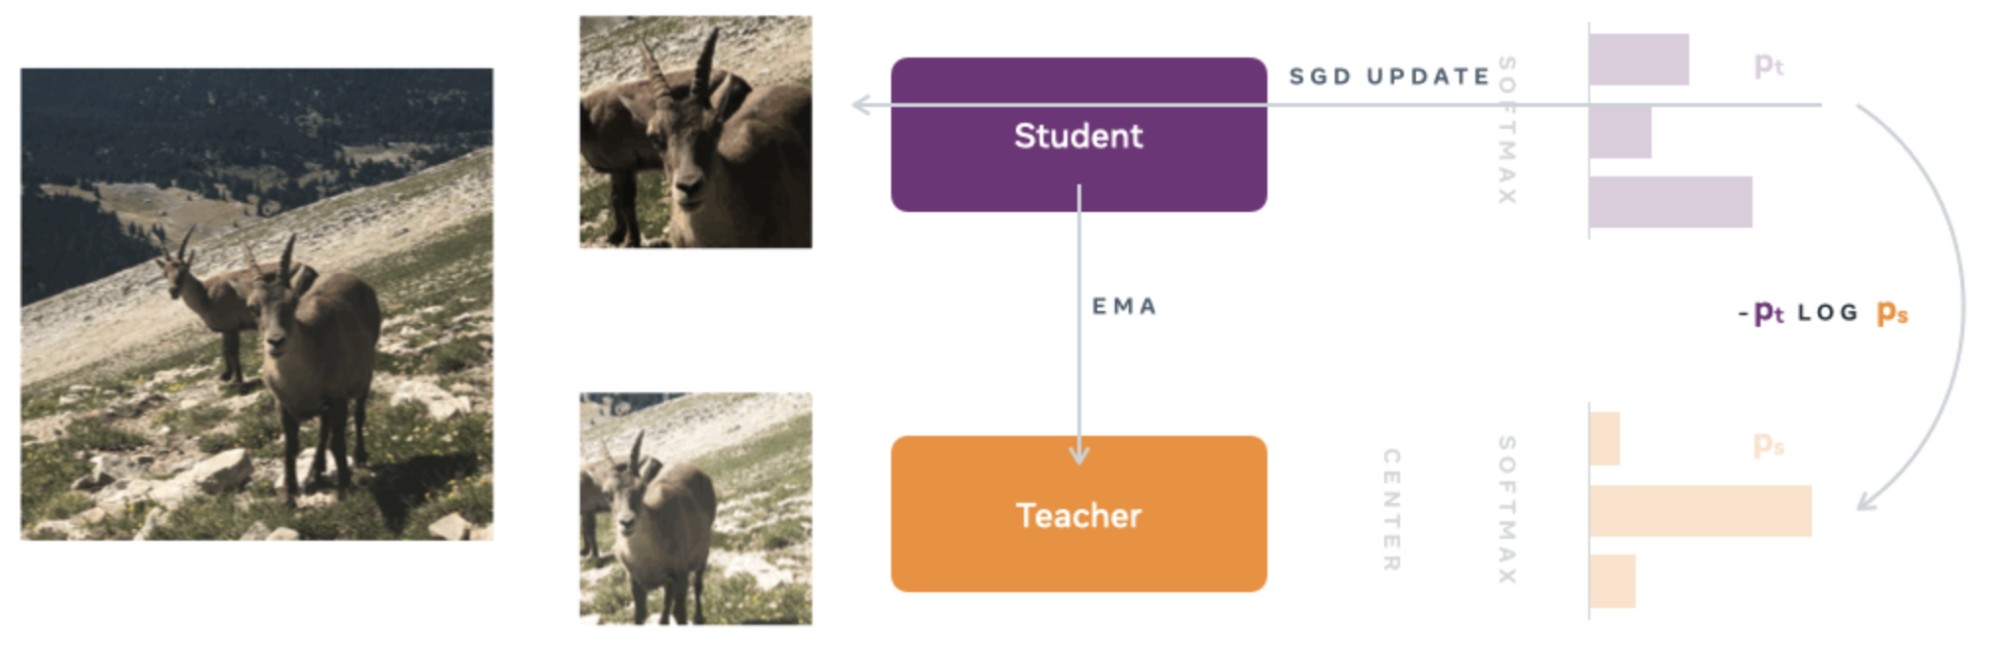
\includegraphics[width=0.9\textwidth]{images/dinov2_teacher_student.png}
	\captionof{figure}{Sơ đồ trực giác của DINOv2: Học sinh dự đoán phân phối đầu ra của giáo viên từ các view khác nhau. Giáo viên được cập nhật bằng trung bình động từ học sinh.}
	\label{fig:dinov2_teacher_student}
\end{center}


\begin{center}
	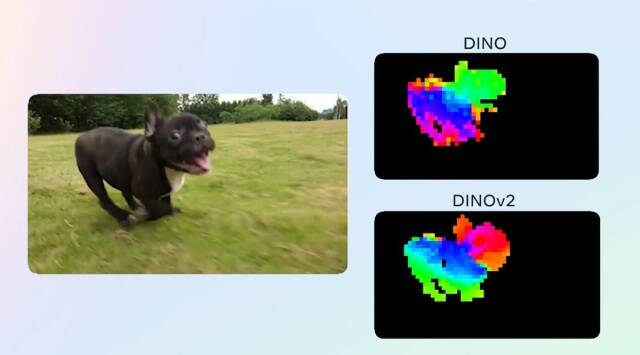
\includegraphics[width=0.9\textwidth]{images/dinov2_semantic_segmentation.jpg}
	\captionof{figure}{Ví dụ về khả năng zero-shot của DINOv2. Các đặc trưng từ DINOv2 có thể được phân cụm một cách đơn giản (ví dụ: bằng k-NN) để tạo ra các mặt nạ phân đoạn ngữ nghĩa chất lượng cao mà không cần bất kỳ sự huấn luyện nào trên tác vụ phân đoạn.}
	\label{fig:dinov2_segmentation}
\end{center}
% Keyword gợi ý: dinov2 zero-shot segmentation, dino self-distillation

\subsubsection{OpenCLIP: Học Biểu diễn Thị giác-Ngôn ngữ Tương phản}
\label{subsubsec:openclip_math}

\textbf{Cơ sở Toán học: Contrastive Learning đa phương thức}  

Cho một batch gồm $N$ cặp $(x_i, t_i)$, với $x_i$ là ảnh và $t_i$ là văn bản tương ứng. CLIP sử dụng hai encoder:
\[
v_i = f_\theta(x_i) \in \mathbb{R}^d, \quad
u_i = g_\phi(t_i) \in \mathbb{R}^d
\]
với $f_\theta$ là Image Encoder (ViT/ResNet), $g_\phi$ là Text Encoder (Transformer). Hai embedding được chuẩn hóa:
\[
\tilde{v}_i = \frac{v_i}{\|v_i\|_2}, \quad \tilde{u}_i = \frac{u_i}{\|u_i\|_2}.
\]

Hàm mất mát InfoNCE đa phương thức:
\[
\mathcal{L}_i = - \log \frac{\exp(\tilde{v}_i \cdot \tilde{u}_i / \tau)}
{\sum_{j=1}^{N} \exp(\tilde{v}_i \cdot \tilde{u}_j / \tau)}, \quad
\mathcal{L} = \frac{1}{2N} \sum_{i=1}^N (\mathcal{L}_i + \mathcal{L}_i^\text{text-to-image})
\]
với $\tau$ là hệ số nhiệt độ (temperature) và $\mathcal{L}_i^\text{text-to-image}$ là hàm tương tự nhưng đổi chiều (text query → image key).

\textbf{Trực giác:}
\begin{itemize}
	\item Các embedding cùng cặp $(x_i, t_i)$ được kéo lại gần nhau trong không gian nhúng, trong khi embedding không cùng cặp bị đẩy ra xa.
	\item Mô hình học được một không gian biểu diễn chung, nơi các đối tượng, khái niệm, và ngữ cảnh đều được mã hóa, cho phép \textbf{zero-shot transfer} sang nhiều tác vụ khác nhau.
	\item OpenCLIP mở rộng ý tưởng này bằng cách:
	\begin{itemize}
		\item Sử dụng \textbf{dữ liệu mở} như LAION-5B để huấn luyện ở quy mô cực lớn.
		\item Cung cấp nhiều cấu hình backbone khác nhau (ResNet, ViT), giúp cộng đồng dễ dàng sử dụng và tùy biến.
	\end{itemize}
\end{itemize}

\textbf{Ứng dụng:}  
Các embedding OpenCLIP trở thành xương sống cho:
\begin{itemize}
	\item Tìm kiếm hình ảnh dựa trên văn bản (Text-to-Image Retrieval)
	\item Tác vụ zero-shot classification
	\item Các hệ thống thị giác-ngôn ngữ như BLIP, Kosmos, và Grounded-SAM
\end{itemize}

\begin{center}
	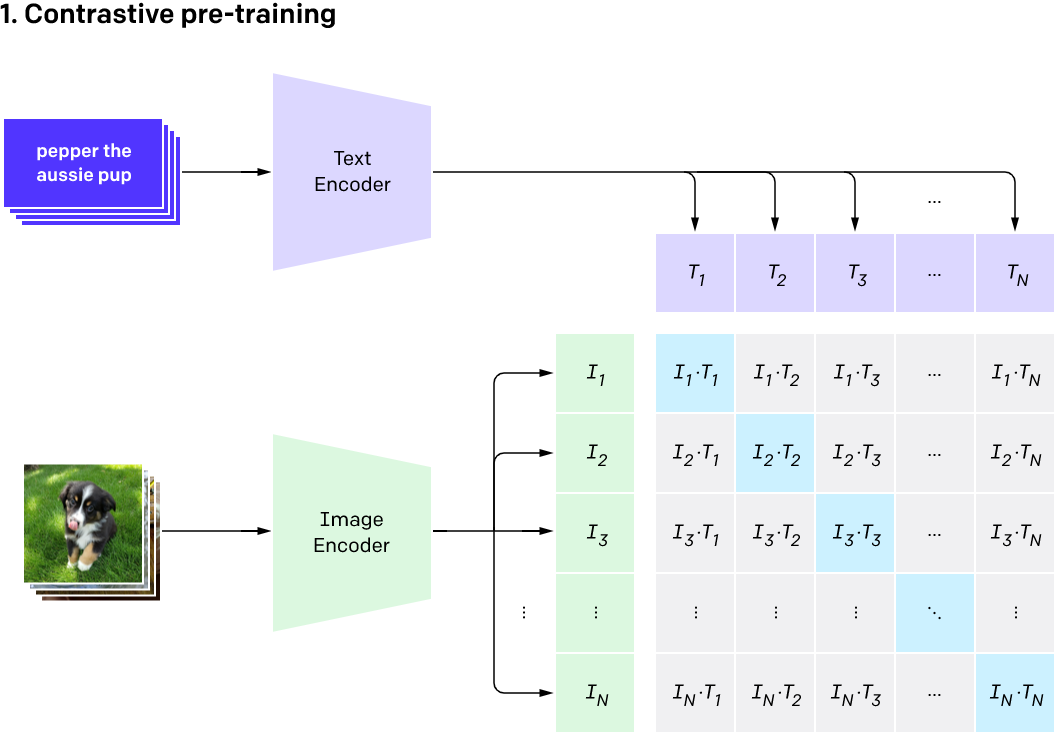
\includegraphics[width=0.9\textwidth]{images/openclip_architecture.png}
	\captionof{figure}{Sơ đồ cơ bản của CLIP/OpenCLIP: hai encoder (ảnh và văn bản) học embedding tương phản trong một không gian nhúng chung.}
	\label{fig:openclip_architecture}
\end{center}

\subsection{I-JEPA: Học Biểu diễn bằng cách Dự đoán trong Không gian Trừu tượng}
\label{subsec:i_jepa}
\textbf{I-JEPA (Image-based Joint-Embedding Predictive Architecture)} \cite{Assran2023} từ Meta AI (đứng đầu bởi Yann LeCun) đại diện cho một triết lý học tự giám sát thứ ba, khác biệt so với cả tương phản và tái tạo pixel.

\textbf{Triết lý cốt lõi: Dự đoán trong Không gian Biểu diễn}
Các phương pháp như MAE buộc mô hình phải tái tạo lại các chi tiết pixel của các patch bị che. Yann LeCun cho rằng đây là một nhiệm vụ không cần thiết và lãng phí tài nguyên tính toán, vì nó buộc mô hình phải quan tâm đến các chi tiết không liên quan đến ngữ nghĩa (ví dụ: kết cấu của từng sợi cỏ).
\begin{itemize}
	\item \textbf{Cơ chế I-JEPA:}
	\begin{enumerate}
		\item Một ảnh được chia thành hai phần: một \textbf{vùng bối cảnh (context block)} lớn và một \textbf{vùng mục tiêu (target block)} nhỏ hơn, bị che.
		\item Cả hai vùng đều được đưa qua một mạng \textbf{giáo viên (teacher encoder)} (được cập nhật bằng trung bình động) để tạo ra các biểu diễn (representations).
		\item Một mạng \textbf{học sinh (student encoder)} chỉ nhìn thấy vùng bối cảnh. Nhiệm vụ của nó là tạo ra một biểu diễn.
		\item Một \textbf{bộ dự đoán (predictor)} nhỏ sau đó nhận biểu diễn của vùng bối cảnh (từ mạng học sinh) và phải \textbf{dự đoán biểu diễn của vùng mục tiêu} (được tạo ra bởi mạng giáo viên).
	\end{enumerate}
	\item \textbf{Mục tiêu:} Thay vì dự đoán các pixel thô, mô hình chỉ cần dự đoán các thông tin ngữ nghĩa, trừu tượng trong không gian biểu diễn. Điều này buộc mô hình phải học các mối quan hệ ngữ cảnh và một mô hình nội tại (internal model) về thế giới.
\end{itemize}

\begin{center}
	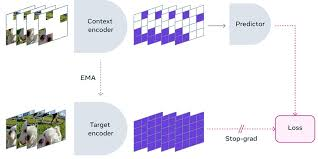
\includegraphics[width=1.0\textwidth]{images/i_jepa_architecture.jpg}
	\captionof{figure}{Sơ đồ kiến trúc của I-JEPA. Mạng học sinh (student) chỉ quan sát vùng bối cảnh và phải dự đoán biểu diễn (representation) của các vùng mục tiêu (target) trong không gian đặc trưng của mạng giáo viên (teacher).}
	\label{fig:i_jepa_architecture}
\end{center}
% Keyword gợi ý: i-jepa architecture, joint embedding predictive architecture

\subsection{Kết luận: Biểu diễn là Ngôn ngữ Mới của AI}
\label{subsec:foundation_representations_conclusion}
DINOv2, OpenCLIP, và I-JEPA, mặc dù sử dụng các phương pháp học khác nhau (tự chưng cất, tương phản đa phương thức, dự đoán trừu tượng), đều hội tụ về một mục tiêu chung: tạo ra một \textbf{không gian nhúng phổ quát và thống nhất}.

Trong kỷ nguyên mới này, các biểu diễn được học bởi các mô hình nền tảng không chỉ là một sản phẩm phụ của quá trình huấn luyện. Chúng đang trở thành một sản phẩm chính, một loại "ngôn ngữ trung gian" của AI thị giác. Các nhà phát triển có thể lấy các bộ mã hóa "đóng gói" này, trích xuất các biểu diễn mạnh mẽ, và sử dụng chúng cho hàng loạt các ứng dụng mà không cần phải huấn luyện lại các mô hình khổng lồ từ đầu.

Câu nói \textit{"Software is eating the world"} đã định hình thập kỷ trước. Trong thập kỷ này, có lẽ câu nói phù hợp sẽ là: \textit{"Representation is the new API"}. Các biểu diễn nền tảng chính là giao diện lập trình ứng dụng cho phép chúng ta xây dựng thế hệ tiếp theo của các hệ thống AI thông minh, linh hoạt và có khả năng hiểu thế giới một cách sâu sắc.

\section*{Tài liệu tham khảo}
\begin{itemize}
	\item[1] Oquab, M., Darcet, T., Moutakanni, T., Vo, H., Szafraniec, M., ... \& Joulin, A. (2023). Dinov2: Learning robust visual features without supervision. \textit{arXiv preprint arXiv:2304.07193}. (Paper gốc giới thiệu DINOv2).
	\item[2] Radford, A., Kim, J. W., Hallacy, C., Ramesh, A., Goh, G., Agarwal, S., ... \& Sutskever, I. (2021). Learning transferable visual models from natural language supervision. In \textit{International Conference on Machine Learning (ICML)}. (Paper gốc về CLIP).
	\item[3] Assran, M., Caron, M., Misra, I., Bojanowski, P., Joulin, A., ... \& Ballas, N. (2023). Self-supervised learning from images with a joint-embedding predictive architecture. In \textit{Proceedings of the IEEE/CVF Conference on Computer Vision and Pattern Recognition (CVPR)}. (Paper gốc giới thiệu I-JEPA).
	\item[4] Caron, M., Touvron, H., Misra, I., Jégou, H., Mairal, J., Bojanowski, P., \& Joulin, A. (2021). Emerging properties in self-supervised vision transformers. In \textit{Proceedings of the IEEE/CVF international conference on computer vision (ICCV)}. (Paper gốc giới thiệu DINO).
	\item[5] He, K., Chen, X., Xie, S., Li, Y., Dollár, P., \& Girshick, R. (2022). Masked autoencoders are scalable vision learners. In \textit{Proceedings of the IEEE/CVF conference on computer vision and pattern recognition (CVPR)}. (Paper về MAE, cung cấp bối cảnh cho các phương pháp học dựa trên masking).
\end{itemize}